\section{Dataset} \label{dataset}

	On the Internet there are few open access datasets for skin cancer classification task, and most of them contain a collection of bad quality images that are not biopsy proven. We read a lot of papers on this task and in most of them researchers had to create a dataset from scratch for the unavailability of a complete dataset composed of quality and biopsy proven images on the web. In most cases they took best images from different sources and they built their own dataset. Recently, some researchers and dermatologists understood the importance of this task and decided to create a new dataset, called HAM10000, that we used on our project. 
	This dataset contains 10015 dermatoscopic images that were collected over a period of 20 years from two different sites, the Department of Dermatology at the Medical University of Vienna, Austria, and the skin cancer practice of Cliff Rosendahl in Queensland, Australia. It includes pigmented lesions from different populations. The Austrian image set consists of lesions of patients referred to a tertiary European referral center specialized for early detection of melanoma in high risk groups. The Australian image set includes lesions from patients of a primary care facility in a high skin cancer incidence area. Dermatoscopic images of both study sites were taken by different devices using polarized and non-polarized dermatoscopy. The set includes representative examples of pigmented skin lesions that are practically relevant. More than 95\% of all lesion encountered during clinical practice will fall into one of the seven diagnostic categories contained in the dataset. In practice, the task of the clinician is to differentiate between malignant and benign lesions, but also to make specific diagnoses because different malignant lesions may be treated in a different way and timeframe. The number of images in the datasets does not correspond to the number of unique lesions, because experts also provided images of the same lesion taken at different magnifications or angles, or with different cameras. This should serve as a natural data-augmentation as it shows random transformations and visualizes both general and local features.
	
	\bigskip
	
	The seven different categories of skin lesions contained in the dataset are:
	
	\paragraph{akiec}
	Actinic Keratoses (Solar Keratoses) and Intraepithelial Carcinoma (Bowen’s disease) are common non-invasive, variants of squamous cell carcinoma that can be treated locally without surgery. There is agreement that these lesions may progress to invasive squamous cell carcinoma. 
	
	\paragraph{bcc}
	Basal cell carcinoma is a common variant of epithelial skin cancer that rarely metastasizes but grows destructively if untreated. 
	
	\paragraph{bkl}
	``Benign keratosis" is a generic class that includes seborrheic keratoses (``senile wart"), solar lentigo and lichen-planus like keratoses (LPLK), which corresponds to a seborrheic keratosis or a solar lentigo with inflammation and regression. From a dermatoscopic view, lichen planus-like keratoses are especially challenging because they can show morphologic features mimicking melanoma and are often biopsied or excised for diagnostic reasons. 
	
	\paragraph{df}
	Dermatofibroma is a benign skin lesion regarded as either a benign proliferation or an inflammatory reaction to minimal trauma. 
	
	\paragraph{nv}
	Melanocytic nevi are benign neoplasms of melanocytes and appear in a myriad of variants, which all are included in this dataset. The variants may differ significantly from a dermatoscopic point of view.
	
	\paragraph{mel}
	Melanoma is a malignant neoplasm derived from melanocytes that may appear in different variants. If excised in an early stage it can be cured by simple surgical excision. 
	
	\paragraph{vasc}
	Vascular skin lesions in the dataset range from cherry angiomas to angiokeratomas and pyogenic granulomas. Hemorrhage is also included in this category.
	
	\bigskip
	
	In Figure \ref{fig:category_samples} is possible to see the difference between these types of skin lesions.
	
	\begin{figure}[H]
		\centering
		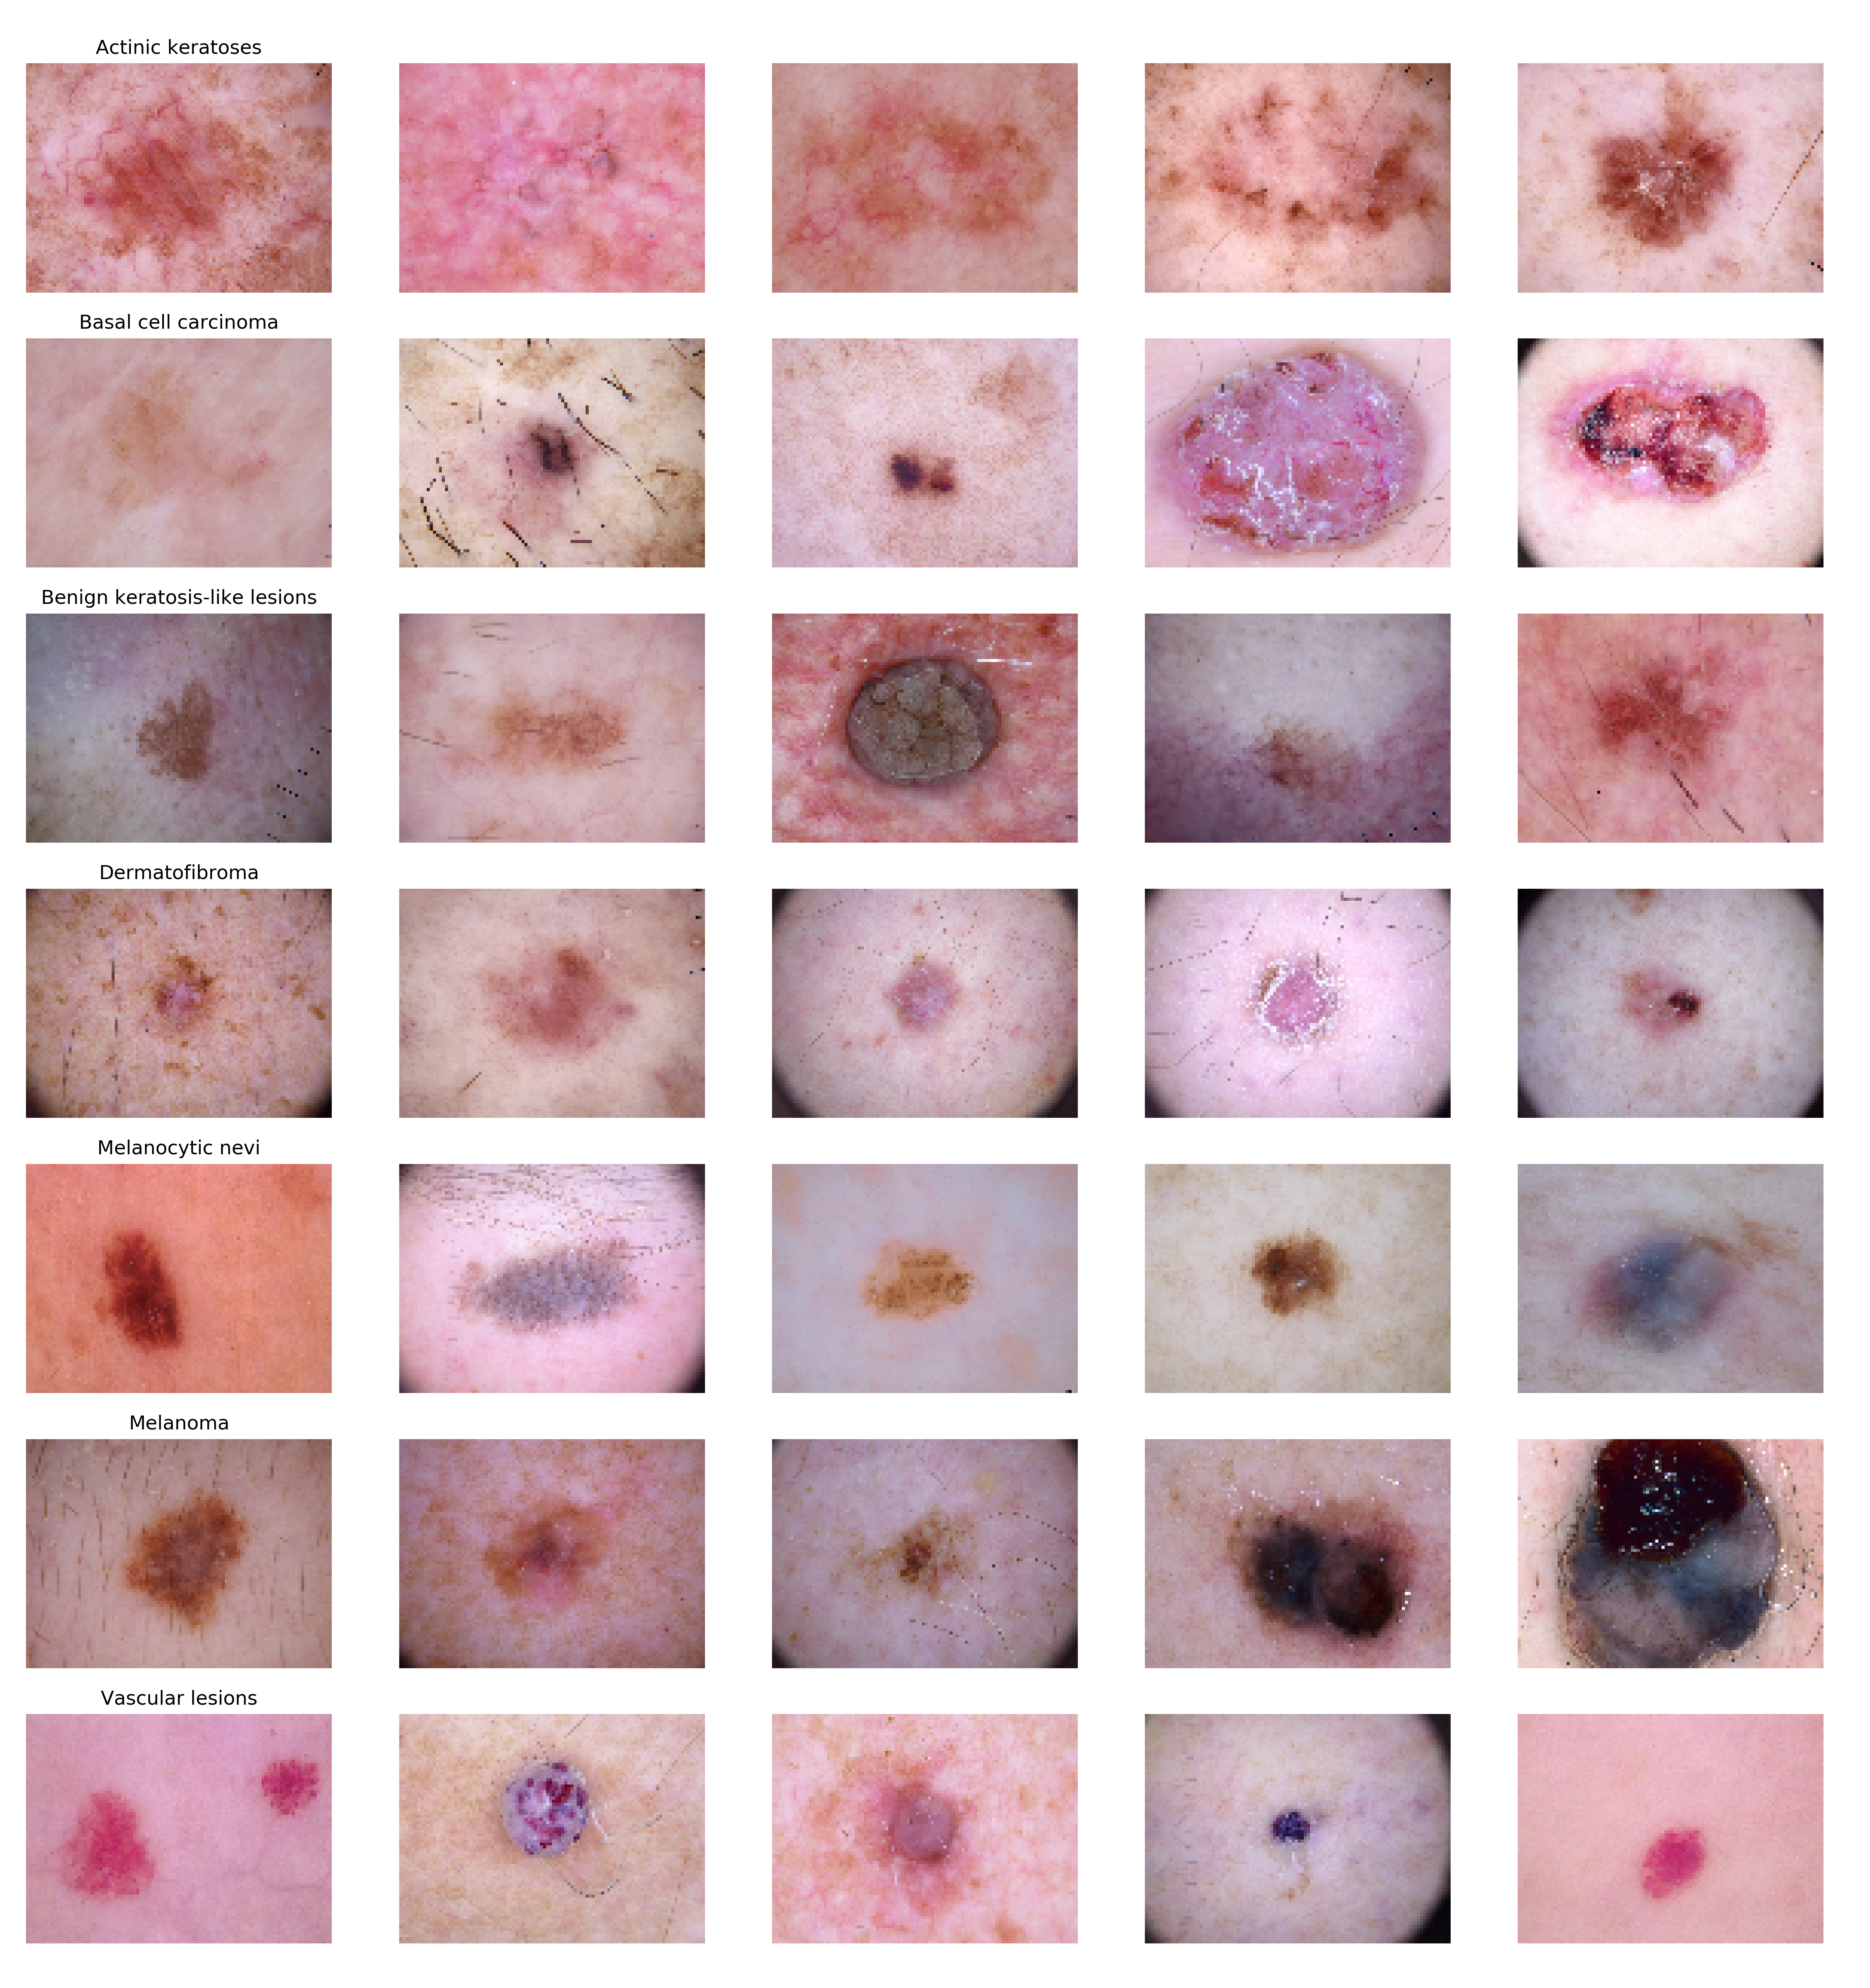
\includegraphics[width=15cm]{images/category_samples.png}
		\caption{Categories of skin lesions in HAM10000}
		\label{fig:category_samples}
	\end{figure}
	
	Imbalanced data is the biggest problem of HAM10000, in fact melanocytic nevi is the majority class with 67\% of examples, instead dermatofibroma is the minority class with only 4\% of examples. In Figure \ref{fig:graph1} is possible to see the distribution of classes. 
	
	\smallskip
	
	Imbalanced data is a common issue of skin cancer datasets and have been a challenge for this project. Initially we thought to find other images to oversample the dataset, but then we turned out that images in the internet are bad in quality and different compared to the images of the HAM10000, so we have decided to keep it at the original version.
	Data preprocessing in this dataset has been limited to the normalization of images and the transformation of labels in one-hot encoded vectors to make the net capable to learn from them. We have decided to split the dataset in 80\% training set and 10\% test set, then we took a 10\% validation set from the training set. We kept this aggressive split because of the limited amount of data, in fact we want our model to learn as much as possible features from the dataset. Images have been resized to 100 x 75 before being supplied to the CNN model. We have decided this specific sizes because experiments showed that the model works better with small resolution images.
	
	\begin{figure}[H]
		\centering
		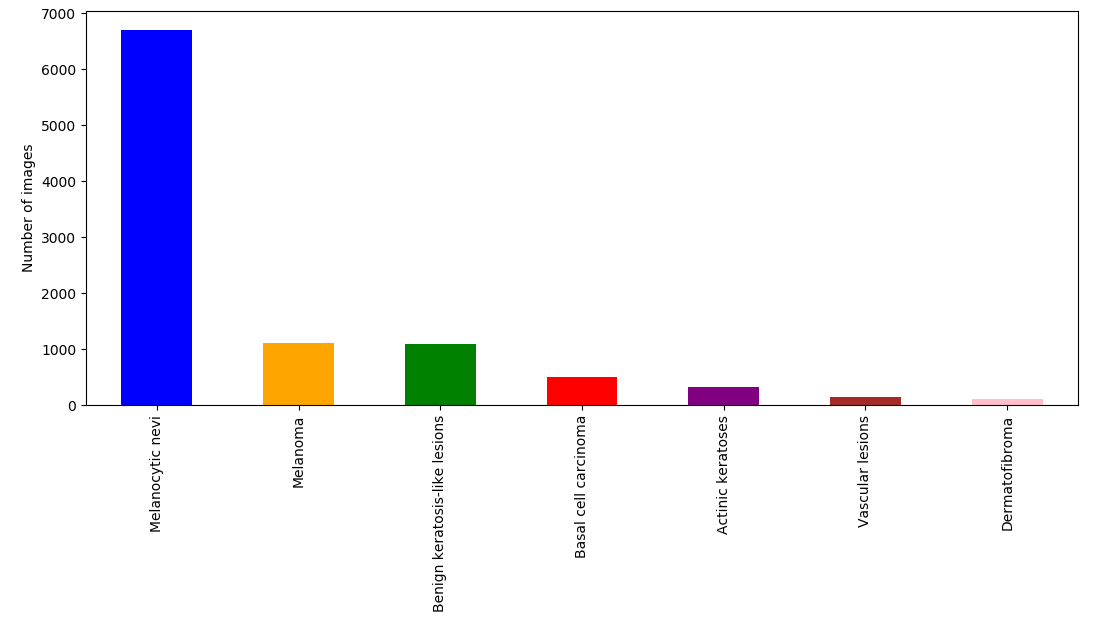
\includegraphics[width=15cm]{images/graph1.png}
		\caption{Distribution of categories in HAM10000}
		\label{fig:graph1}
	\end{figure}